% Options for packages loaded elsewhere
\PassOptionsToPackage{unicode}{hyperref}
\PassOptionsToPackage{hyphens}{url}
%
\documentclass[
]{article}
\usepackage{amsmath,amssymb}
\usepackage{iftex}
\ifPDFTeX
  \usepackage[T1]{fontenc}
  \usepackage[utf8]{inputenc}
  \usepackage{textcomp} % provide euro and other symbols
\else % if luatex or xetex
  \usepackage{unicode-math} % this also loads fontspec
  \defaultfontfeatures{Scale=MatchLowercase}
  \defaultfontfeatures[\rmfamily]{Ligatures=TeX,Scale=1}
\fi
\usepackage{lmodern}
\ifPDFTeX\else
  % xetex/luatex font selection
\fi
% Use upquote if available, for straight quotes in verbatim environments
\IfFileExists{upquote.sty}{\usepackage{upquote}}{}
\IfFileExists{microtype.sty}{% use microtype if available
  \usepackage[]{microtype}
  \UseMicrotypeSet[protrusion]{basicmath} % disable protrusion for tt fonts
}{}
\makeatletter
\@ifundefined{KOMAClassName}{% if non-KOMA class
  \IfFileExists{parskip.sty}{%
    \usepackage{parskip}
  }{% else
    \setlength{\parindent}{0pt}
    \setlength{\parskip}{6pt plus 2pt minus 1pt}}
}{% if KOMA class
  \KOMAoptions{parskip=half}}
\makeatother
\usepackage{xcolor}
\usepackage[margin=1in]{geometry}
\usepackage{color}
\usepackage{fancyvrb}
\newcommand{\VerbBar}{|}
\newcommand{\VERB}{\Verb[commandchars=\\\{\}]}
\DefineVerbatimEnvironment{Highlighting}{Verbatim}{commandchars=\\\{\}}
% Add ',fontsize=\small' for more characters per line
\usepackage{framed}
\definecolor{shadecolor}{RGB}{248,248,248}
\newenvironment{Shaded}{\begin{snugshade}}{\end{snugshade}}
\newcommand{\AlertTok}[1]{\textcolor[rgb]{0.94,0.16,0.16}{#1}}
\newcommand{\AnnotationTok}[1]{\textcolor[rgb]{0.56,0.35,0.01}{\textbf{\textit{#1}}}}
\newcommand{\AttributeTok}[1]{\textcolor[rgb]{0.13,0.29,0.53}{#1}}
\newcommand{\BaseNTok}[1]{\textcolor[rgb]{0.00,0.00,0.81}{#1}}
\newcommand{\BuiltInTok}[1]{#1}
\newcommand{\CharTok}[1]{\textcolor[rgb]{0.31,0.60,0.02}{#1}}
\newcommand{\CommentTok}[1]{\textcolor[rgb]{0.56,0.35,0.01}{\textit{#1}}}
\newcommand{\CommentVarTok}[1]{\textcolor[rgb]{0.56,0.35,0.01}{\textbf{\textit{#1}}}}
\newcommand{\ConstantTok}[1]{\textcolor[rgb]{0.56,0.35,0.01}{#1}}
\newcommand{\ControlFlowTok}[1]{\textcolor[rgb]{0.13,0.29,0.53}{\textbf{#1}}}
\newcommand{\DataTypeTok}[1]{\textcolor[rgb]{0.13,0.29,0.53}{#1}}
\newcommand{\DecValTok}[1]{\textcolor[rgb]{0.00,0.00,0.81}{#1}}
\newcommand{\DocumentationTok}[1]{\textcolor[rgb]{0.56,0.35,0.01}{\textbf{\textit{#1}}}}
\newcommand{\ErrorTok}[1]{\textcolor[rgb]{0.64,0.00,0.00}{\textbf{#1}}}
\newcommand{\ExtensionTok}[1]{#1}
\newcommand{\FloatTok}[1]{\textcolor[rgb]{0.00,0.00,0.81}{#1}}
\newcommand{\FunctionTok}[1]{\textcolor[rgb]{0.13,0.29,0.53}{\textbf{#1}}}
\newcommand{\ImportTok}[1]{#1}
\newcommand{\InformationTok}[1]{\textcolor[rgb]{0.56,0.35,0.01}{\textbf{\textit{#1}}}}
\newcommand{\KeywordTok}[1]{\textcolor[rgb]{0.13,0.29,0.53}{\textbf{#1}}}
\newcommand{\NormalTok}[1]{#1}
\newcommand{\OperatorTok}[1]{\textcolor[rgb]{0.81,0.36,0.00}{\textbf{#1}}}
\newcommand{\OtherTok}[1]{\textcolor[rgb]{0.56,0.35,0.01}{#1}}
\newcommand{\PreprocessorTok}[1]{\textcolor[rgb]{0.56,0.35,0.01}{\textit{#1}}}
\newcommand{\RegionMarkerTok}[1]{#1}
\newcommand{\SpecialCharTok}[1]{\textcolor[rgb]{0.81,0.36,0.00}{\textbf{#1}}}
\newcommand{\SpecialStringTok}[1]{\textcolor[rgb]{0.31,0.60,0.02}{#1}}
\newcommand{\StringTok}[1]{\textcolor[rgb]{0.31,0.60,0.02}{#1}}
\newcommand{\VariableTok}[1]{\textcolor[rgb]{0.00,0.00,0.00}{#1}}
\newcommand{\VerbatimStringTok}[1]{\textcolor[rgb]{0.31,0.60,0.02}{#1}}
\newcommand{\WarningTok}[1]{\textcolor[rgb]{0.56,0.35,0.01}{\textbf{\textit{#1}}}}
\usepackage{graphicx}
\makeatletter
\def\maxwidth{\ifdim\Gin@nat@width>\linewidth\linewidth\else\Gin@nat@width\fi}
\def\maxheight{\ifdim\Gin@nat@height>\textheight\textheight\else\Gin@nat@height\fi}
\makeatother
% Scale images if necessary, so that they will not overflow the page
% margins by default, and it is still possible to overwrite the defaults
% using explicit options in \includegraphics[width, height, ...]{}
\setkeys{Gin}{width=\maxwidth,height=\maxheight,keepaspectratio}
% Set default figure placement to htbp
\makeatletter
\def\fps@figure{htbp}
\makeatother
\setlength{\emergencystretch}{3em} % prevent overfull lines
\providecommand{\tightlist}{%
  \setlength{\itemsep}{0pt}\setlength{\parskip}{0pt}}
\setcounter{secnumdepth}{-\maxdimen} % remove section numbering
\ifLuaTeX
  \usepackage{selnolig}  % disable illegal ligatures
\fi
\IfFileExists{bookmark.sty}{\usepackage{bookmark}}{\usepackage{hyperref}}
\IfFileExists{xurl.sty}{\usepackage{xurl}}{} % add URL line breaks if available
\urlstyle{same}
\hypersetup{
  pdftitle={TDE},
  hidelinks,
  pdfcreator={LaTeX via pandoc}}

\title{TDE}
\author{}
\date{\vspace{-2.5em}2023-09-25}

\begin{document}
\maketitle

\hypertarget{exam-style-questions}{%
\section{Exam style questions}\label{exam-style-questions}}

\hypertarget{algorithmic-instructions}{%
\subsection{Algorithmic instructions}\label{algorithmic-instructions}}

(Pasted from an actual exam, we will use some of the parameters later)

\begin{itemize}
\tightlist
\item
  All the numerical values required need to be put on an A4 sheet and
  uploaded, alongside the required plots.
\item
  For all computations based on permutation/resampling, as well as split
  conformal, use B = 1000 replicates, and seed = 1991.
\item
  Both for confidence and prediction intervals, as well as tests, set
  \(\alpha\) = 0.05.
\item
  When reporting a test result, please specify H0, H1 , the P-value and
  the corresponding conclusion.
\item
  When reporting confidence/prediction intervals, always provide upper
  and lower bound.
\end{itemize}

\hypertarget{exercise-1}{%
\subsubsection{Exercise 1}\label{exercise-1}}

Dr.~Yorkhamikis has been long retired from the academy. Time has
definitely passed since he left his Associate Professor job at a
prestigious university in Milan to go back to his hometown in Greece,
where he currently raises cattle. He still keeps his quantitative
approach though, and has instructed his employee to gather data relative
to three key quantities concerning the milk of his cows (filename\_
milk\_samples\_1.Rds \_Assume observations to be independent between
them

\begin{Shaded}
\begin{Highlighting}[]
\NormalTok{ALPHA }\OtherTok{=} \FloatTok{0.05} \CommentTok{\# set values as required}
\NormalTok{B }\OtherTok{=} \FloatTok{1e4}

\CommentTok{\# load data set}
\NormalTok{df.latte }\OtherTok{\textless{}{-}} \FunctionTok{readRDS}\NormalTok{(}\AttributeTok{file =} \StringTok{"data/milk\_samples\_1.Rds"}\NormalTok{)}
\FunctionTok{library}\NormalTok{(aplpack)}
\CommentTok{\# of course, the bagplot is the multivariate extension of the boxplot}
\CommentTok{\# since we are dealing with 3 dimensions, we use a bagplot matrix where at each square we have a bagplot of two measures}
\NormalTok{bagplot\_matrix }\OtherTok{\textless{}{-}}\NormalTok{ aplpack}\SpecialCharTok{::}\FunctionTok{bagplot.pairs}\NormalTok{(df.latte)}
\end{Highlighting}
\end{Shaded}

\includegraphics{TDEs_files/figure-latex/unnamed-chunk-2-1.pdf} To
identify the outliers, the procedure is the following:

\begin{itemize}
\tightlist
\item
  For each pair of measures (dimensions):

  \begin{itemize}
  \tightlist
  \item
    Obtain the bagplot (each bagplot is bi-dimensional).
  \item
    Label as outliers points which lie outside the fence \footnote{You
      may ask yourselves why the function does not require the method to
      compute the depth. The bagplot uses the Tukey depth to recognise
      the deepest 50\% of the data set}
  \item
    Append the indices of those outliers to the general outlier list
  \end{itemize}
\end{itemize}

\begin{Shaded}
\begin{Highlighting}[]
\NormalTok{OUTLIER.INDICES }\OtherTok{=} \FunctionTok{as.numeric}\NormalTok{(}\DecValTok{0}\NormalTok{)  }\CommentTok{\# initialise the vector containing the outlier indices}

\NormalTok{df.first.comb }\OtherTok{=}\NormalTok{ df.latte[,}\FunctionTok{c}\NormalTok{(}\DecValTok{1}\NormalTok{,}\DecValTok{2}\NormalTok{)]  }\CommentTok{\# take the first two measures}
\CommentTok{\# retrieve the outliers from the bagplot of the comparison of the first two mearues}
\NormalTok{bagplot.first.comb }\OtherTok{=} \FunctionTok{bagplot}\NormalTok{(df.first.comb)}
\end{Highlighting}
\end{Shaded}

\includegraphics{TDEs_files/figure-latex/unnamed-chunk-3-1.pdf}

\begin{Shaded}
\begin{Highlighting}[]
\NormalTok{outliers.first }\OtherTok{=}\NormalTok{ bagplot.first.comb}\SpecialCharTok{$}\NormalTok{pxy.outlier  }\CommentTok{\# N.B. this function retrieves the rows which are outliers, NOT the indices}

\CommentTok{\# we thus extract the outlier indices (this is just a copy{-}paste of the first laboratory)}
\NormalTok{indices.one }\OtherTok{=} \FunctionTok{which}\NormalTok{(}\FunctionTok{apply}\NormalTok{(df.first.comb,}\DecValTok{1}\NormalTok{,}\ControlFlowTok{function}\NormalTok{(x) }\FunctionTok{all}\NormalTok{(x }\SpecialCharTok{\%in\%}\NormalTok{ outliers.first)))}

\CommentTok{\# combine elements}
\NormalTok{OUTLIER.INDICES }\OtherTok{=} \FunctionTok{c}\NormalTok{(OUTLIER.INDICES, indices.one)}
\NormalTok{OUTLIER.INDICES}
\end{Highlighting}
\end{Shaded}

\begin{verbatim}
##  [1]   0   1  45  83  95 177 188 200 219 234 257 260 264 266 275 295 301 351 368
## [20] 369 373 374 375 376 377 378 379 380 381 382
\end{verbatim}

\begin{Shaded}
\begin{Highlighting}[]
\CommentTok{\# we continue the analysis by comparing the other dimensions}
\NormalTok{df.second }\OtherTok{=}\NormalTok{ df.latte[,}\FunctionTok{c}\NormalTok{(}\DecValTok{1}\NormalTok{,}\DecValTok{3}\NormalTok{)]}
\NormalTok{bagplot.second.comb }\OtherTok{=} \FunctionTok{bagplot}\NormalTok{(df.second)}
\end{Highlighting}
\end{Shaded}

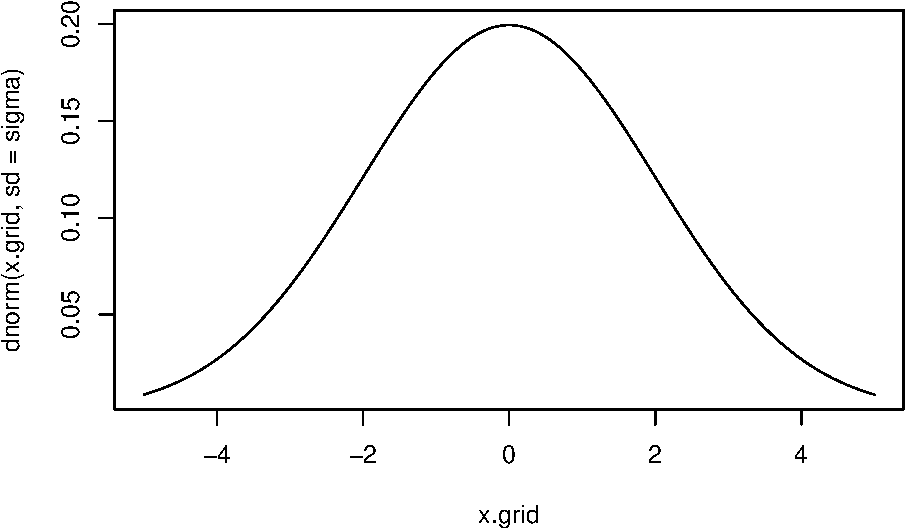
\includegraphics{TDEs_files/figure-latex/unnamed-chunk-4-1.pdf}

\begin{Shaded}
\begin{Highlighting}[]
\NormalTok{outliers.second }\OtherTok{=}\NormalTok{ bagplot.second.comb}\SpecialCharTok{$}\NormalTok{pxy.outlier}
\NormalTok{indices.two }\OtherTok{=} \FunctionTok{which}\NormalTok{(}\FunctionTok{apply}\NormalTok{(df.second,}\DecValTok{1}\NormalTok{,}\ControlFlowTok{function}\NormalTok{(x) }\FunctionTok{all}\NormalTok{(x }\SpecialCharTok{\%in\%}\NormalTok{ outliers.second)))}

\CommentTok{\# set "global" variables}
\end{Highlighting}
\end{Shaded}

\begin{enumerate}
\def\labelenumi{\arabic{enumi}.}
\tightlist
\item
  Dr.~Yorkhamikis distrusts his employee, and is convinced there are
  observations that were not written down correctly and thus are not
  coherent with the true data. Devise a graphic method to retrieve such
  entries looking at the three measures relative to the milk and report
  the incoherent values.
\end{enumerate}

\begin{Shaded}
\begin{Highlighting}[]
\FunctionTok{library}\NormalTok{(aplpack)}
\NormalTok{bagplot\_matrix }\OtherTok{\textless{}{-}} \FunctionTok{bagplot.pairs}\NormalTok{(df.latte)}
\end{Highlighting}
\end{Shaded}

\includegraphics{TDEs_files/figure-latex/unnamed-chunk-5-1.pdf} First
pair:

\begin{Shaded}
\begin{Highlighting}[]
\NormalTok{outlier\_indices }\OtherTok{\textless{}{-}} \FunctionTok{as.numeric}\NormalTok{(}\DecValTok{0}\NormalTok{)}

\CommentTok{\#selecting the desired comb}
\NormalTok{df.first.comb }\OtherTok{\textless{}{-}}\NormalTok{ df.latte[,}\FunctionTok{c}\NormalTok{(}\DecValTok{1}\NormalTok{,}\DecValTok{2}\NormalTok{)]}

\CommentTok{\#computing the bagplot}
\NormalTok{bagplot.first.comb }\OtherTok{\textless{}{-}} \FunctionTok{bagplot}\NormalTok{(df.first.comb)}
\end{Highlighting}
\end{Shaded}

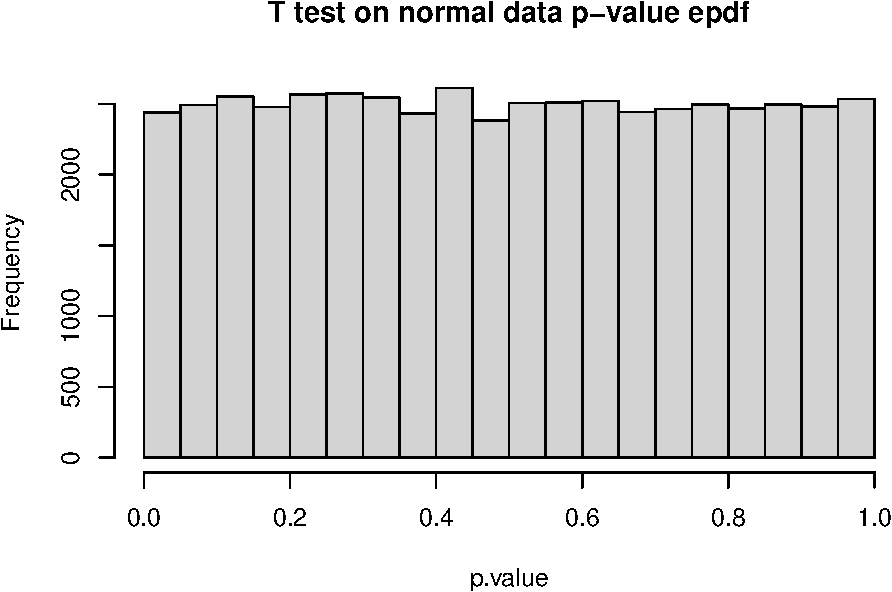
\includegraphics{TDEs_files/figure-latex/unnamed-chunk-6-1.pdf}

\begin{Shaded}
\begin{Highlighting}[]
\CommentTok{\#identifying the outliers and their indices}
\NormalTok{outliers.first }\OtherTok{\textless{}{-}}\NormalTok{ bagplot.first.comb}\SpecialCharTok{$}\NormalTok{pxy.outlier}
\NormalTok{indices.first }\OtherTok{\textless{}{-}} \FunctionTok{which}\NormalTok{(}\FunctionTok{apply}\NormalTok{(df.first.comb,}\DecValTok{1}\NormalTok{,}\ControlFlowTok{function}\NormalTok{(x) }\FunctionTok{all}\NormalTok{(x }\SpecialCharTok{\%in\%}\NormalTok{ outliers.first)))}

\CommentTok{\#adding to the outliers indices vector}
\NormalTok{outlier\_indices }\OtherTok{\textless{}{-}} \FunctionTok{c}\NormalTok{(outlier\_indices, outliers.first)}
\end{Highlighting}
\end{Shaded}

Second pair:

\begin{Shaded}
\begin{Highlighting}[]
\CommentTok{\#selecting the desired comb}
\NormalTok{df.second.comb }\OtherTok{\textless{}{-}}\NormalTok{ df.latte[,}\FunctionTok{c}\NormalTok{(}\DecValTok{1}\NormalTok{,}\DecValTok{3}\NormalTok{)]}

\CommentTok{\#computing the bagplot}
\NormalTok{bagplot.second.comb }\OtherTok{\textless{}{-}} \FunctionTok{bagplot}\NormalTok{(df.second.comb)}
\end{Highlighting}
\end{Shaded}

\includegraphics{TDEs_files/figure-latex/unnamed-chunk-7-1.pdf}

\begin{Shaded}
\begin{Highlighting}[]
\CommentTok{\#identifying the outliers and their indices}
\NormalTok{outliers.second }\OtherTok{\textless{}{-}}\NormalTok{ bagplot.second.comb}\SpecialCharTok{$}\NormalTok{pxy.outlier}
\NormalTok{indices.second }\OtherTok{\textless{}{-}} \FunctionTok{which}\NormalTok{(}\FunctionTok{apply}\NormalTok{(df.second.comb,}\DecValTok{1}\NormalTok{,}\ControlFlowTok{function}\NormalTok{(x) }\FunctionTok{all}\NormalTok{(x }\SpecialCharTok{\%in\%}\NormalTok{ outliers.second)))}

\CommentTok{\#adding to the outliers indices vector}
\NormalTok{outlier\_indices }\OtherTok{\textless{}{-}} \FunctionTok{c}\NormalTok{(outlier\_indices, outliers.second)}
\end{Highlighting}
\end{Shaded}

Third pair

\begin{Shaded}
\begin{Highlighting}[]
\CommentTok{\#First pair}
\NormalTok{outlier\_indices }\OtherTok{\textless{}{-}} \FunctionTok{as.numeric}\NormalTok{(}\DecValTok{0}\NormalTok{)}

\CommentTok{\#selecting the desired comb}
\NormalTok{df.third.comb }\OtherTok{\textless{}{-}}\NormalTok{ df.latte[,}\FunctionTok{c}\NormalTok{(}\DecValTok{2}\NormalTok{,}\DecValTok{3}\NormalTok{)]}

\CommentTok{\#computing the bagplot}
\NormalTok{bagplot.third.comb }\OtherTok{\textless{}{-}} \FunctionTok{bagplot}\NormalTok{(df.third.comb)}
\end{Highlighting}
\end{Shaded}

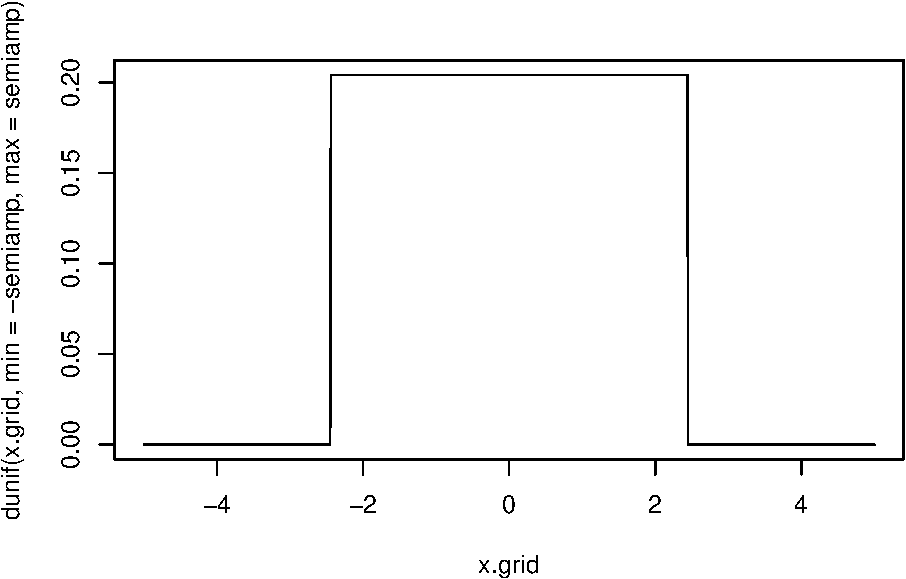
\includegraphics{TDEs_files/figure-latex/unnamed-chunk-8-1.pdf}

\begin{Shaded}
\begin{Highlighting}[]
\CommentTok{\#identifying the outliers and their indices}
\NormalTok{outliers.third }\OtherTok{\textless{}{-}}\NormalTok{ bagplot.third.comb}\SpecialCharTok{$}\NormalTok{pxy.outlier}
\NormalTok{indices.third }\OtherTok{\textless{}{-}} \FunctionTok{which}\NormalTok{(}\FunctionTok{apply}\NormalTok{(df.third.comb,}\DecValTok{1}\NormalTok{,}\ControlFlowTok{function}\NormalTok{(x) }\FunctionTok{all}\NormalTok{(x }\SpecialCharTok{\%in\%}\NormalTok{ outliers.third)))}

\CommentTok{\#adding to the outliers indices vector}
\NormalTok{outlier\_indices }\OtherTok{\textless{}{-}} \FunctionTok{c}\NormalTok{(outlier\_indices, outliers.third)}
\end{Highlighting}
\end{Shaded}

\begin{enumerate}
\def\labelenumi{\arabic{enumi}.}
\setcounter{enumi}{1}
\tightlist
\item
  The distrust of the Dr.~has been increasing a lot lately. He now also
  suspects that the second half of the observations were invented by his
  employee, who supposedly preferred to make the data up and have a nap.
  Dr.~Yorkhamikis says this will be evident in the median of the PH of
  the second half of the observations, which should be quite different
  from the median of the industry standard which is \(n\). Implement a
  pertinent (two-sided) statistical test relative to the median of the
  PH of the second half of the observations and write down your
  conclusions.
\end{enumerate}

\begin{Shaded}
\begin{Highlighting}[]
\NormalTok{df.purged }\OtherTok{\textless{}{-}}\NormalTok{ df.latte[}\SpecialCharTok{{-}}\NormalTok{outlier\_indices,]}
\NormalTok{PH }\OtherTok{\textless{}{-}}\NormalTok{ df.purged}\SpecialCharTok{$}\NormalTok{Native\_pH}

\NormalTok{PH }\OtherTok{\textless{}{-}}\NormalTok{ PH[}\FunctionTok{ceiling}\NormalTok{(}\FunctionTok{length}\NormalTok{(PH)}\SpecialCharTok{/}\DecValTok{2}\NormalTok{)}\SpecialCharTok{:}\FunctionTok{length}\NormalTok{(PH)]}
\end{Highlighting}
\end{Shaded}

Assumptions: - observations are i.i.d. - under H0, the count of points
higher than 6 should be distributed as a Binomial(, 0.5)

H0: median(PH) = 6 H1: median(PH) != 6

The test statistic is going to be \[
max(w,w*)
\] w: count of values higher than 6

\begin{Shaded}
\begin{Highlighting}[]
\NormalTok{median.H0 }\OtherTok{\textless{}{-}} \DecValTok{6}
\NormalTok{n }\OtherTok{\textless{}{-}} \FunctionTok{length}\NormalTok{(PH)}

\NormalTok{w }\OtherTok{\textless{}{-}} \FunctionTok{sum}\NormalTok{(PH }\SpecialCharTok{\textgreater{}}\NormalTok{ median.H0)}
\NormalTok{w.star }\OtherTok{\textless{}{-}} \FunctionTok{max}\NormalTok{(}\FunctionTok{c}\NormalTok{(w, n }\SpecialCharTok{{-}}\NormalTok{ w))}

\FunctionTok{plot}\NormalTok{(}\DecValTok{0}\SpecialCharTok{:}\NormalTok{n, }\FunctionTok{dbinom}\NormalTok{(}\DecValTok{0}\SpecialCharTok{:}\NormalTok{n, n, }\FloatTok{0.5}\NormalTok{))}
\FunctionTok{abline}\NormalTok{(}\AttributeTok{v =} \FunctionTok{c}\NormalTok{(w, n }\SpecialCharTok{{-}}\NormalTok{ w), }\AttributeTok{col=}\StringTok{"red"}\NormalTok{)}
\end{Highlighting}
\end{Shaded}

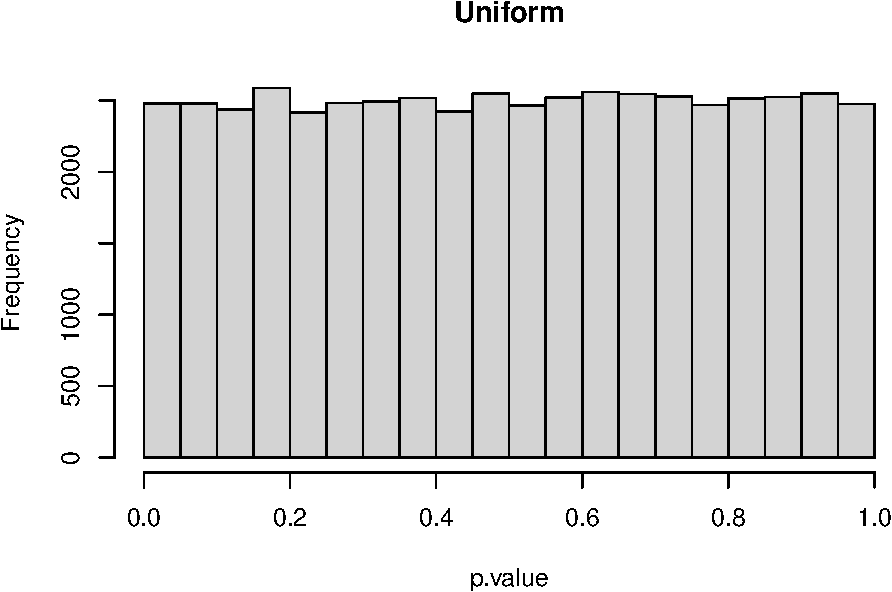
\includegraphics{TDEs_files/figure-latex/unnamed-chunk-10-1.pdf}

\begin{Shaded}
\begin{Highlighting}[]
\NormalTok{p.value }\OtherTok{\textless{}{-}} \DecValTok{2}\SpecialCharTok{*}\NormalTok{(}\DecValTok{1} \SpecialCharTok{{-}} \FunctionTok{pbinom}\NormalTok{(w.star}\DecValTok{{-}1}\NormalTok{,n,}\FloatTok{0.5}\NormalTok{)) }
\end{Highlighting}
\end{Shaded}

\begin{enumerate}
\def\labelenumi{\arabic{enumi}.}
\setcounter{enumi}{2}
\tightlist
\item
  Repeat the test for the .25th quantile, using for \(H_0\) the .25th
  quantile equals the one of the first half (first 160-something rows)
  of the population.
\end{enumerate}

\begin{Shaded}
\begin{Highlighting}[]
\NormalTok{PH.first.half }\OtherTok{\textless{}{-}}\NormalTok{ df.purged}\SpecialCharTok{$}\NormalTok{Native\_pH[}\DecValTok{1}\SpecialCharTok{:}\FunctionTok{ceiling}\NormalTok{(}\FunctionTok{length}\NormalTok{(df.purged}\SpecialCharTok{$}\NormalTok{Native\_pH)}\SpecialCharTok{/}\DecValTok{2}\NormalTok{)]}

\NormalTok{H0.value }\OtherTok{\textless{}{-}} \FunctionTok{quantile}\NormalTok{(PH.first.half, }\FloatTok{0.25}\NormalTok{)}
\end{Highlighting}
\end{Shaded}

H0: 25th\_quantile(PH) = 6.59 H1: 25th\_quantile(PH) != 6.59

\begin{Shaded}
\begin{Highlighting}[]
\NormalTok{n }\OtherTok{\textless{}{-}} \FunctionTok{length}\NormalTok{(PH)}

\NormalTok{w }\OtherTok{\textless{}{-}} \FunctionTok{sum}\NormalTok{(PH }\SpecialCharTok{\textgreater{}}\NormalTok{ H0.value)}

\FunctionTok{plot}\NormalTok{(}\DecValTok{0}\SpecialCharTok{:}\NormalTok{n, }\FunctionTok{dbinom}\NormalTok{(}\DecValTok{0}\SpecialCharTok{:}\NormalTok{n, n, }\FloatTok{0.25}\NormalTok{))}
\FunctionTok{abline}\NormalTok{(}\AttributeTok{v =} \FunctionTok{c}\NormalTok{(w, n }\SpecialCharTok{{-}}\NormalTok{ w), }\AttributeTok{col=}\StringTok{"red"}\NormalTok{)}
\end{Highlighting}
\end{Shaded}

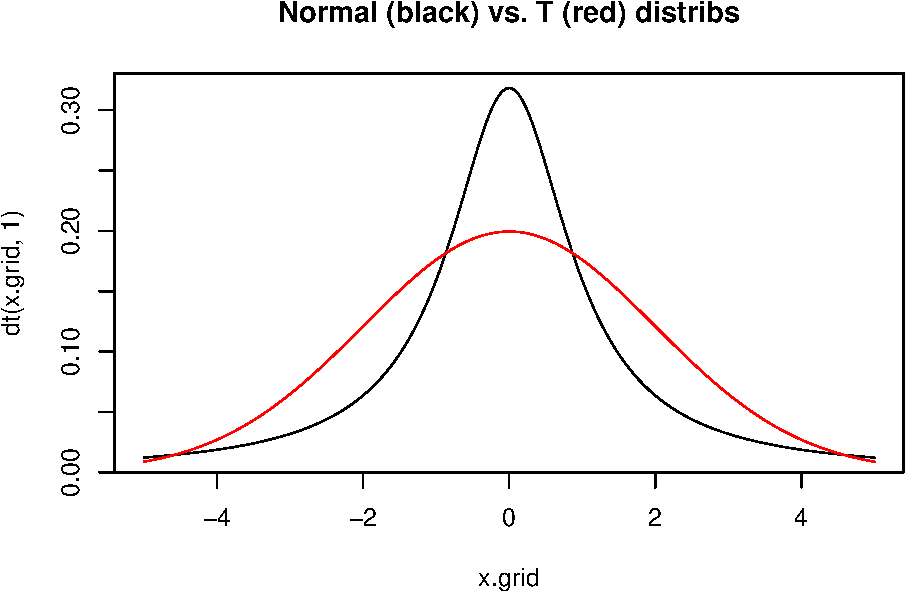
\includegraphics{TDEs_files/figure-latex/unnamed-chunk-12-1.pdf}

\begin{Shaded}
\begin{Highlighting}[]
\NormalTok{OUTLIER.INDICES }\OtherTok{\textless{}{-}} \FunctionTok{c}\NormalTok{(OUTLIER.INDICES, indices.two)}


\NormalTok{df.third }\OtherTok{=}\NormalTok{ df.latte[,}\FunctionTok{c}\NormalTok{(}\DecValTok{2}\NormalTok{,}\DecValTok{3}\NormalTok{)]}
\NormalTok{bagplot.third.comb }\OtherTok{=} \FunctionTok{bagplot}\NormalTok{(df.third)}
\end{Highlighting}
\end{Shaded}

\includegraphics{TDEs_files/figure-latex/unnamed-chunk-13-1.pdf}

\begin{Shaded}
\begin{Highlighting}[]
\NormalTok{outliers.third }\OtherTok{=}\NormalTok{ bagplot.third.comb}\SpecialCharTok{$}\NormalTok{pxy.outlier}
\NormalTok{indices.three }\OtherTok{=} \FunctionTok{which}\NormalTok{(}\FunctionTok{apply}\NormalTok{(df.third,}\DecValTok{1}\NormalTok{,}\ControlFlowTok{function}\NormalTok{(x) }\FunctionTok{all}\NormalTok{(x }\SpecialCharTok{\%in\%}\NormalTok{ outliers.third)))}

\NormalTok{OUTLIER.INDICES }\OtherTok{\textless{}{-}} \FunctionTok{c}\NormalTok{(OUTLIER.INDICES, indices.three)}
\FunctionTok{unique}\NormalTok{(OUTLIER.INDICES) }\CommentTok{\# retrieve the unique entries}
\end{Highlighting}
\end{Shaded}

\begin{verbatim}
##  [1]   0   1  45  83  95 177 188 200 219 234 257 260 264 266 275 295 301 351 368
## [20] 369 373 374 375 376 377 378 379 380 381 382   2   6  20  37  49 144 185 281
## [39] 303  35 105 233
\end{verbatim}

\begin{enumerate}
\def\labelenumi{\arabic{enumi}.}
\setcounter{enumi}{1}
\tightlist
\item
  \emph{The distrust of the Dr.~has been increasing a lot lately. He now
  also suspects that the second half of the observations were invented
  by his employee, who supposedly preferred to make the data up and have
  a nap. Dr.~Yorkhamikis says this will be evident in the median of the
  PH of the second half of the observations (of course look only at the
  ones who were written down correctly), which should be quite different
  from the median of the industry standard which is} \(6.5\)
  \emph{Implement a pertinent nonparametric statistical test \footnote{When
    this TDE was created, we had only studied the sign tests, so there
    is only one coherent possibility. In the exam, we will be more
    specific, since you could think of a sign test, a Mann-Whitney
    signed rank test, a permutation test, a Bootstrap test\ldots{}} to
  evaluate whether PH of the second half of the observations is
  different from the industry standard and write down your conclusions}.
\end{enumerate}

We first firstly manipulate the data frame to obtain the relevant data.

\begin{Shaded}
\begin{Highlighting}[]
\CommentTok{\# remove the outliers}
\NormalTok{df.purged }\OtherTok{=}\NormalTok{ df.latte[}\SpecialCharTok{{-}}\NormalTok{OUTLIER.INDICES,]}
\CommentTok{\# focus on the measure under question}
\NormalTok{PH }\OtherTok{\textless{}{-}}\NormalTok{ df.purged}\SpecialCharTok{$}\NormalTok{Native\_pH}
\CommentTok{\# retrieve the second half of the observations}
\NormalTok{PH }\OtherTok{\textless{}{-}}\NormalTok{ PH[}\FunctionTok{ceiling}\NormalTok{(}\FunctionTok{length}\NormalTok{(PH)}\SpecialCharTok{/}\DecValTok{2}\NormalTok{)}\SpecialCharTok{:}\FunctionTok{length}\NormalTok{(PH)]}
\end{Highlighting}
\end{Shaded}

The used test is a sign test. Let \(X\) be the R.V. representing the
measure of the milk's PH. We test: \[
H_0 = \{ \mathbb{P}[X > 6.5]  = 0.5 \}
\] \emph{versus} \[
H_1 = \{ \mathbb{P} [X > 6.5] \neq 0.5 \}
\] (i.e.~if the population's median is \(6.5\) vs.~it is not).

The test statistic is going to be: \[w* := max(w, N-w)\] where \[
w := \sum_{i=1}^{N} \mathcal{1}_{\{x_i > 6.5 \}}
\] That is, the count of data points that are higher than the
hypothesised median (naturally \(x_i\) denotes the \(i\)th statistical
unit present in the sample and \(N\) is the sample size). We choose the
maximum between \(w\) and \(N-w\) since the value will be symmetric with
respect to the median under \(H_0\) (which is \(0.5 * N\))

Assumptions:

\begin{itemize}
\tightlist
\item
  Observations are i.i.d.
\item
  Under H0, the test statistic has the following property:
\end{itemize}

\$\$ w* \stackrel{H_0}{\sim} Binomial(N, .25)

\$\$

\begin{Shaded}
\begin{Highlighting}[]
\NormalTok{median.h0 }\OtherTok{\textless{}{-}} \FloatTok{6.5}
\NormalTok{n }\OtherTok{\textless{}{-}} \FunctionTok{length}\NormalTok{(PH)}
\NormalTok{w }\OtherTok{\textless{}{-}} \FunctionTok{sum}\NormalTok{(PH }\SpecialCharTok{\textgreater{}}\NormalTok{ median.h0)}
\NormalTok{w.star }\OtherTok{\textless{}{-}} \FunctionTok{max}\NormalTok{(}\FunctionTok{c}\NormalTok{(w, n }\SpecialCharTok{{-}}\NormalTok{ w))}

\CommentTok{\# plot distribution under H\_0}
\FunctionTok{plot}\NormalTok{(}\DecValTok{0}\SpecialCharTok{:}\NormalTok{n, }\FunctionTok{dbinom}\NormalTok{(}\DecValTok{0}\SpecialCharTok{:}\NormalTok{n, n, }\FloatTok{0.5}\NormalTok{))}
\CommentTok{\# add value of test statistic obtained with the sample}
\FunctionTok{abline}\NormalTok{(}\AttributeTok{v =} \FunctionTok{c}\NormalTok{(w, n}\SpecialCharTok{{-}}\NormalTok{w), }\AttributeTok{col=}\StringTok{\textquotesingle{}red\textquotesingle{}}\NormalTok{)}
\end{Highlighting}
\end{Shaded}

\includegraphics{TDEs_files/figure-latex/unnamed-chunk-15-1.pdf}

We calculate the p-value \(p\) in the following way: \[
p = \mathbb{P}_{H_0}[W^* \geq w^* ] = 2 \sum_{n=w*}^N \binom{N}{n}0.5^n(1-0.5)^{N-n}
\] (we calculate the mass of the right tail of the binomial distribution
using the value of the statistic obtained with the sample and multiply
it by two since it is symmetric about \(0.5n\))

\begin{Shaded}
\begin{Highlighting}[]
\NormalTok{p.value }\OtherTok{\textless{}{-}} \DecValTok{2}\SpecialCharTok{*}\NormalTok{(}\DecValTok{1} \SpecialCharTok{{-}} \FunctionTok{pbinom}\NormalTok{(w.star}\DecValTok{{-}1}\NormalTok{, n, }\FloatTok{0.5}\NormalTok{, }\AttributeTok{lower.tail =}\NormalTok{ T) )}
\NormalTok{p.value}
\end{Highlighting}
\end{Shaded}

\begin{verbatim}
## [1] 0
\end{verbatim}

Which can be computed manually:

\begin{Shaded}
\begin{Highlighting}[]
\NormalTok{bin.pmf }\OtherTok{\textless{}{-}} \ControlFlowTok{function}\NormalTok{(x) (}\FunctionTok{choose}\NormalTok{(n, x) }\SpecialCharTok{*} \FloatTok{0.5}\SpecialCharTok{\^{}}\NormalTok{x }\SpecialCharTok{*}\NormalTok{(}\DecValTok{1}\FloatTok{{-}0.5}\NormalTok{)}\SpecialCharTok{**}\NormalTok{(n}\SpecialCharTok{{-}}\NormalTok{x))}

\NormalTok{p.value }\OtherTok{\textless{}{-}} \DecValTok{2} \SpecialCharTok{*}\NormalTok{ (}\DecValTok{1} \SpecialCharTok{{-}} \FunctionTok{sum}\NormalTok{(}\FunctionTok{sapply}\NormalTok{(}\DecValTok{1}\SpecialCharTok{:}\NormalTok{(w.star}\DecValTok{{-}1}\NormalTok{),  }\AttributeTok{FUN=}\NormalTok{bin.pmf ))}
\NormalTok{                )}
\NormalTok{p.value}
\end{Highlighting}
\end{Shaded}

\begin{verbatim}
## [1] -6.217249e-15
\end{verbatim}

Moreover, is tantamount to \footnote{execute \emph{?pbinom} and look the
  lower.tail argument}:

\begin{Shaded}
\begin{Highlighting}[]
\NormalTok{p.value }\OtherTok{\textless{}{-}} \DecValTok{2}\SpecialCharTok{*}\NormalTok{( }\FunctionTok{pbinom}\NormalTok{(w.star}\DecValTok{{-}1}\NormalTok{, n, }\FloatTok{0.5}\NormalTok{, }\AttributeTok{lower.tail =}\NormalTok{ F) )}
\NormalTok{p.value}
\end{Highlighting}
\end{Shaded}

\begin{verbatim}
## [1] 7.910334e-43
\end{verbatim}

Or much more simply:

\begin{Shaded}
\begin{Highlighting}[]
\FunctionTok{binom.test}\NormalTok{(}\FunctionTok{sum}\NormalTok{(w), n, }\AttributeTok{p=}\FloatTok{0.5}\NormalTok{, }\AttributeTok{alternative=}\StringTok{"two.sided"}\NormalTok{,}
           \AttributeTok{conf.level =} \DecValTok{1}\SpecialCharTok{{-}}\NormalTok{ALPHA)}
\end{Highlighting}
\end{Shaded}

\begin{verbatim}
## 
##  Exact binomial test
## 
## data:  sum(w) and n
## number of successes = 166, number of trials = 171, p-value < 2.2e-16
## alternative hypothesis: true probability of success is not equal to 0.5
## 95 percent confidence interval:
##  0.9330861 0.9904391
## sample estimates:
## probability of success 
##              0.9707602
\end{verbatim}

The p-value is practically zero (which is coherent with the fact the
value we obtained of the statistic is positioned at the tails of the
distribution), meaning we reject \(H_0\) in favour of \(H_1\): we have
statistical evidence to assert that the median of the second half of the
(clean) observations is different from the industry standard.
(Alternatively, we could state that the confidence interval obtained
from the Binomial distribution does not contain the value under \(H_0\)
so we reject \(H_0\)).

\begin{enumerate}
\def\labelenumi{\arabic{enumi}.}
\setcounter{enumi}{2}
\tightlist
\item
  \emph{Repeat the test for the .25th quantile, using for} \(H_0\)
  \emph{the .25th quantile equals the one of the first half (first
  160-something rows) of the population.}
\end{enumerate}

We first obtain the first half of the actual (i.e.~without outliers)
observations relative to the PH, and retrieve the value we are going to
test against.

\begin{Shaded}
\begin{Highlighting}[]
\NormalTok{PH.first.half }\OtherTok{=}\NormalTok{ df.purged}\SpecialCharTok{$}\NormalTok{Native\_pH[}\DecValTok{1}\SpecialCharTok{:}\FunctionTok{ceiling}\NormalTok{(}\FunctionTok{length}\NormalTok{(df.purged}\SpecialCharTok{$}\NormalTok{Native\_pH)}\SpecialCharTok{/}\DecValTok{2}\NormalTok{)]}
\NormalTok{H0.value }\OtherTok{=} \FunctionTok{quantile}\NormalTok{(PH.first.half, .}\DecValTok{25}\NormalTok{)}
\end{Highlighting}
\end{Shaded}

The test statistic is\^{}{[}we could also just use the count of winners
against \(c_0\) and have under \(H_0\) a \(Binomial(n, 0.75)\), as we
would expect \(75%
\) of data to be higher than the \(25th\) quantile : \[
w := n-\sum_{i=1}^N \mathcal{1}_{\{ x_i > c_0\}}
\] We test \[
H_0 = \{\mathbb{P}[X > 0.25] = c_0 \}
\] \emph{versus} \[
H_1 = \{\mathbb{P}[X > 0.25] \neq c_0 \}
\] Having that: \$\$ w \stackrel{H_0}{\sim} Binomial(N, .25)

\$\$

\begin{Shaded}
\begin{Highlighting}[]
\NormalTok{n }\OtherTok{\textless{}{-}} \FunctionTok{length}\NormalTok{(PH) }
\NormalTok{w }\OtherTok{\textless{}{-}}\NormalTok{ n }\SpecialCharTok{{-}} \FunctionTok{sum}\NormalTok{(PH }\SpecialCharTok{\textgreater{}}\NormalTok{ H0.value)}

\FunctionTok{plot}\NormalTok{(}\DecValTok{0}\SpecialCharTok{:}\NormalTok{n, }\FunctionTok{dbinom}\NormalTok{(}\DecValTok{0}\SpecialCharTok{:}\NormalTok{n, n, }\FloatTok{0.25}\NormalTok{))}
\FunctionTok{abline}\NormalTok{(}\AttributeTok{v =} \FunctionTok{c}\NormalTok{(w), }\AttributeTok{col=}\StringTok{\textquotesingle{}red\textquotesingle{}}\NormalTok{)}
\end{Highlighting}
\end{Shaded}

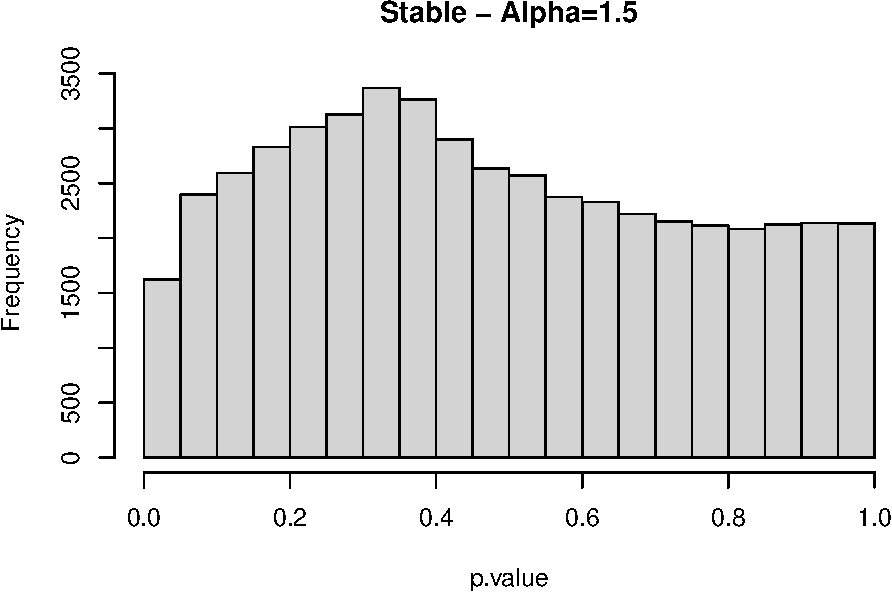
\includegraphics{TDEs_files/figure-latex/unnamed-chunk-21-1.pdf} Since
the Binomial distribution is no longer symmetric (whenever its
probability parameter is different from \(0.5\)), the calculation of the
p-value is more complex, \emph{i.e.} we cannot take one tail's mass and
double it anymore \footnote{See
  \url{https://en.wikipedia.org/wiki/Binomial_test} for details}

As we saw before, once we build the statistic, we can apply the
function:

\begin{Shaded}
\begin{Highlighting}[]
\FunctionTok{binom.test}\NormalTok{(w, n, }\FloatTok{0.25}\NormalTok{, }\AttributeTok{alternative=}\StringTok{"two.sided"}\NormalTok{, }\AttributeTok{conf.level =} \DecValTok{1}\SpecialCharTok{{-}}\NormalTok{ALPHA)}
\end{Highlighting}
\end{Shaded}

\begin{verbatim}
## 
##  Exact binomial test
## 
## data:  w and n
## number of successes = 43, number of trials = 171, p-value = 1
## alternative hypothesis: true probability of success is not equal to 0.25
## 95 percent confidence interval:
##  0.1883513 0.3233982
## sample estimates:
## probability of success 
##               0.251462
\end{verbatim}

We fail to reject \(H_0\): we have no statistical evidence to suggest
the \(.25th\) quantile of the second half of the sample is different
from that of the first half.

\begin{enumerate}
\def\labelenumi{\arabic{enumi}.}
\setcounter{enumi}{3}
\tightlist
\item
  \emph{Mention the theoretical properties of the test you have used.}
\end{enumerate}

The sign test does not make assumptions of the underlying distribution
of the data sample.

Under \(H_0\), the distribution of the test statistic is Binomial. This
is a discrete distribution, whence the sample size \(n\) determines
achievable levels of significance that can be built without a
randomisation strategy.

If the underlying distribution of the sample is symmetric, and its first
moment exists, then this test is tantamount to testing a hypothesised
mean (the median matches the mean).

As \(n\) grows, the distribution under \(H_0\) of the statistic
converges to \(N(\frac{n}{2}, \frac{n}{4})\)

It supports a one-sided version (focusing on the pertinent tail), and
the testing of a certain value of the quantile (although the symmetry of
the binomial distribution is lost)

Extensions to discrete and ordinal data are available.

\end{document}
